\documentclass[a4paper, 10pt]{article}

\usepackage{amsmath}
\usepackage{siunitx}
\usepackage{graphicx}
\usepackage[T1]{fontenc}
\usepackage[utf8]{inputenc}
\usepackage[english]{babel}
\usepackage[sc]{mathpazo}
\usepackage{color}

% Various spacing parameters
\usepackage{microtype}
\usepackage[margin=3.5cm]{geometry}
\linespread{1}
\parindent 0pt
\parskip 4pt

% Helping functions
\newcommand{\pdiff}[2]{\frac{\partial #1}{\partial #2}} % Partial derivative

% Spacing inside description environment
\usepackage{enumitem}
\setlist[description]{style=multiline,leftmargin=.8cm,parsep=4pt}

\title{Fluid Dynamics + Turbulence (fall 2018)\\Homework Problems II}
\author{}
\date{}

%----------------------------------------------------------------------------------------

\begin{document}
\maketitle

\large{
\textbf{Posted:}
\today

\bigskip
\textbf{Deadline:}
September 18 (Tuesday) at 08:30 am (on Blackboard).
}


\bigskip

\section*{Homework problem 2: Surface bump or dip in a shallow river flow?} 
Consider an ideal two-dimensional shallow river flow over a small bump at the river bed; see sketch.
\begin{figure}[h!]
	\centering
	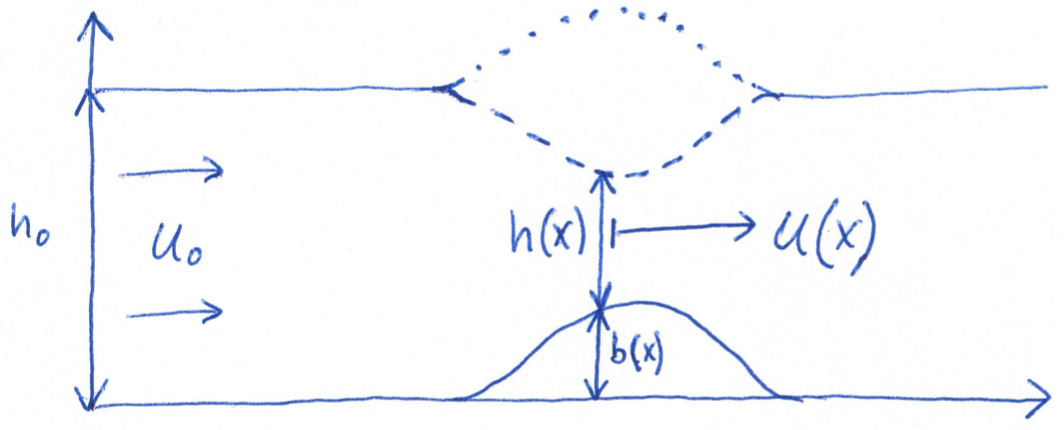
\includegraphics[width=.7\textwidth]{bump.png}
\end{figure}

{\bf (a)} Explain the two conservation laws: 
\begin{eqnarray}
	u_0 h_0 &=& u(x) h(x) \; , \\
	\frac{u_0^2}{2} + g h_0 &=& \frac{u^2(x)}{2} + g \left( b(x) + h(x) \right) \; .
\end{eqnarray}
{\bf (b)} Equations (1) and (2) are two equations for the two unknown functions $h(x)$ and $u(x)$. Eliminate $u(x)$ and derive an equation only for $h(x)$. Show that this equation is consistently solved by $h(x)=h_0$ when $b(x)=0$. In order to solve the equation also for $b(x)>0$, assume the bump $b(x)\ll h_0$ and the change of river surface height $\Delta h(x) = h(x)-h_0\ll h_0$ to be small. Derive the solution
\begin{equation}
	\Delta h(x) = \frac{b(x)}{\left(\frac{u_0^2}{gh_0}-1\right)}
\end{equation}
by keeping first-order terms in small $b(x)/h_0$ and $\Delta h(x)/h_0$ in a consistent way. \newline

{\bf (c)} Use equation (3) in the two limits $u_0^2\ll gh_0$ and $u_ 0^2 \gg g h_0$ to explain when a surface bump or dip occurs. \newline

{\bf (d)} What is the catch with equation (3) when $u_0^2\approx gh_0$? \newline

{\bf (e)} Use the numbers $b_\mathrm{max}=\SI{0.1}{m}$, $h_0=\SI{1}{m}$, $g=\SI{9.81}{m/s^2}$ to calculate the extremum of $\Delta h(x)$ for $u_0=\SI{1}{m/s}$ and $u_0=\SI{10}{m/s}$.


\end{document}